\documentclass[aspectratio=169]{beamer}

\usepackage[utf8]{inputenc}
\usepackage[english]{babel}
\usepackage{booktabs}
\usepackage{array}
\usepackage{listings}
\usepackage{tikz}
\usetikzlibrary{arrows.meta,positioning,shapes.geometric,shapes.multipart,calc,decorations.pathreplacing}

\graphicspath{{logo/}{../logo/}}

\definecolor{ForestGreen}{RGB}{22,100,70}
\definecolor{SoftGreen}{RGB}{229,244,235}
\definecolor{SoftBlue}{RGB}{226,239,255}
\definecolor{SoftOrange}{RGB}{255,241,220}
\definecolor{SoftPurple}{RGB}{239,231,255}
\definecolor{SoftGray}{RGB}{245,247,250}

\newcolumntype{L}[1]{>{\raggedright\arraybackslash}p{#1}}

\mode<presentation>{
  \usetheme{Ilmenau}
  \usecolortheme{spruce}
  \usefonttheme{professionalfonts}
  \setbeamertemplate{navigation symbols}{}
  \setbeamertemplate{headline}{}
  \setbeamertemplate{caption}[numbered]
  \setbeamercolor{institute in head/foot}{fg=ForestGreen}
}

\lstdefinestyle{pseudo}{
  language={},
  basicstyle=\ttfamily\scriptsize,
  keywordstyle=\color{blue!75!black}\bfseries,
  morekeywords={FUNCTION,INPUT,OUTPUT,IF,THEN,ELSE,RETURN,FOR,EACH,IN,TO,DO,
    WHILE,NONE,TRUE,FALSE,CREATE,APPEND,INSERT,REMOVE,PUSH,POP,PEEK,
    ENQUEUE,DEQUEUE,LENGTH,CLASS},
  numbers=none,
  showstringspaces=false,
  keepspaces=true,
  columns=fullflexible,
  breaklines=true,
  frame=single,
  rulecolor=\color{ForestGreen!60},
  backgroundcolor=\color{SoftBlue!35},
  tabsize=4
}

\newcommand{\pseudonumberstyle}{%
  \tiny\ifnum\value{lstnumber}>0\color{gray}\else\color{white}\fi}
\lstdefinestyle{pseudonumbered}{
  style=pseudo,
  numbers=left,
  firstnumber=-2,
  numberstyle=\pseudonumberstyle,
  numbersep=6pt,
  numberblanklines=false
}

\tikzset{
  cell/.style={draw=ForestGreen,fill=SoftGreen,thick,minimum width=0.88cm,
    minimum height=0.72cm,align=center},
  active/.style={draw=orange!75!black,fill=SoftOrange,very thick,
    minimum width=0.88cm,minimum height=0.72cm,align=center},
  found/.style={draw=purple!70!black,fill=SoftPurple,very thick,
    minimum width=0.88cm,minimum height=0.72cm,align=center},
  process/.style={draw=ForestGreen,rounded corners,fill=SoftGreen,thick,
    minimum height=0.9cm,text width=2.7cm,align=center},
  nodebox/.style={draw=ForestGreen,fill=SoftGreen,thick,rectangle split,
    rectangle split parts=2,minimum height=0.75cm,align=center},
  dnode/.style={draw=ForestGreen,fill=SoftGreen,thick,rectangle split,
    rectangle split horizontal,rectangle split parts=3,minimum height=0.78cm,align=center},
  arrow/.style={-Latex,very thick,ForestGreen},
  orangearrow/.style={-Latex,very thick,orange!80!black}
}

\title[TOKT11105 -- Lecture 5]{Data Structures and Algorithms in Python\\
Lecture 5: Data Structures}
\subtitle{Part 2: Arrays and Linked Lists}
\author{Faculty of Data Science and Artificial Intelligence}
\institute{National Economics University}
\date{}

\AtBeginSection[]{
  \begin{frame}[plain]
    \begin{center}
      \vfill
      {\color{ForestGreen}\large\bfseries SECTION \insertsectionnumber}
      \vspace{0.8em}
      {\color{ForestGreen}\rule{0.68\textwidth}{1.2pt}}
      \vspace{1.1em}
      {\usebeamerfont{section title}\color{ForestGreen}\LARGE\bfseries
        \parbox{0.86\textwidth}{\centering\insertsectionhead\par}}
      \vspace{1.1em}
      {\color{ForestGreen}\rule{0.68\textwidth}{1.2pt}}
      \vfill
    \end{center}
  \end{frame}
}

\begin{document}

\begin{frame}[plain]
  \setbeamercolor{block body example}{bg=ForestGreen,fg=white}
  \begin{center}
    \begin{beamercolorbox}[wd=\textwidth,sep=1pt,center,rounded=true,shadow=true]{block body example}
      \IfFileExists{logo_slide.png}{\includegraphics[width=0.27\textwidth]{logo_slide.png}}{{\vspace{0.7em}\Large\bfseries FDA -- NEU\vspace{0.7em}}}
    \end{beamercolorbox}
  \end{center}
  \vspace{-0.25em}
  \titlepage
\end{frame}

\logo{\IfFileExists{logo_fda.png}{\includegraphics[width=0.8cm]{logo_fda.png}}{}}
\setbeamercolor{footline upper}{bg=ForestGreen!22,fg=ForestGreen!85!black}
\setbeamercolor{footline lower}{bg=ForestGreen,fg=white}
\setbeamertemplate{footline}{%
  \leavevmode
  \hbox{%
    \begin{beamercolorbox}[wd=.50\paperwidth,ht=2.35ex,dp=.75ex,
      leftskip=1em]{footline upper}
      Faculty of Data Science and Artificial Intelligence
    \end{beamercolorbox}%
    \begin{beamercolorbox}[wd=.50\paperwidth,ht=2.35ex,dp=.75ex,
      rightskip=1em plus1fil]{footline upper}
      \hfill National Economics University
    \end{beamercolorbox}%
  }
  \hbox{%
    \begin{beamercolorbox}[wd=.72\paperwidth,ht=2.35ex,dp=.75ex,
      leftskip=1em]{footline lower}
      \insertshorttitle
    \end{beamercolorbox}%
    \begin{beamercolorbox}[wd=.28\paperwidth,ht=2.35ex,dp=.75ex,
      rightskip=1em plus1fil]{footline lower}
      \hfill Slide \insertframenumber/\inserttotalframenumber
    \end{beamercolorbox}%
  }
}

\begin{frame}{Part 2: Table of Contents}
\small
\begin{enumerate}
  \item \textbf{Sequences and Representations}
  \item \textbf{Arrays and Dynamic Arrays}
  \item \textbf{Linked Lists}
  \item \textbf{Traversing and Updating a Singly Linked List}
  \item \textbf{Comparing Array-Based and Linked Structures}
\end{enumerate}
\end{frame}

\begin{frame}{Learning outcomes for Part 2}
  By the end of this part, students should be able to:
  \begin{enumerate}
    \item Distinguish logical sequence order from physical memory layout.
    \item Explain arrays, dynamic arrays, and Python lists at a conceptual level.
    \item Describe singly, doubly, and circular linked lists.
    \item Trace traversal, search, insertion, and deletion in a singly linked list.
    \item Compare array-based and linked representations by operation cost.
  \end{enumerate}
\end{frame}

% =============================================================
\section{Sequences and Representations}
% =============================================================

\begin{frame}{A sequence can be represented in different ways}
\small
\begin{block}{Logical view}
A sequence stores items in an order:
\[
10,\;20,\;30,\;40.
\]
But the computer can represent this logical order in different ways.
\end{block}

\begin{columns}[T,onlytextwidth]
\begin{column}{0.48\textwidth}
\begin{exampleblock}{Array-based representation}
\centering
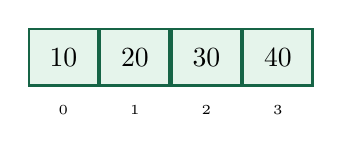
\begin{tikzpicture}[node distance=0pt]
  \node[cell] (a0) {10};
  \node[cell,right=of a0] (a1) {20};
  \node[cell,right=of a1] (a2) {30};
  \node[cell,right=of a2] (a3) {40};
  \node[below=0.12cm of a0,font=\tiny] {0};
  \node[below=0.12cm of a1,font=\tiny] {1};
  \node[below=0.12cm of a2,font=\tiny] {2};
  \node[below=0.12cm of a3,font=\tiny] {3};
\end{tikzpicture}

\vspace{0.25em}
Consecutive positions and direct indexing.
\end{exampleblock}
\end{column}

\begin{column}{0.48\textwidth}
\begin{exampleblock}{Link-based representation}
\centering
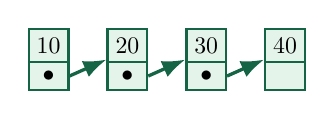
\begin{tikzpicture}[node distance=0.55cm,scale=0.86,transform shape]
  \node[nodebox] (n1) {10\nodepart{second}$\bullet$};
  \node[nodebox,right=of n1] (n2) {20\nodepart{second}$\bullet$};
  \node[nodebox,right=of n2] (n3) {30\nodepart{second}$\bullet$};
  \node[nodebox,right=of n3] (n4) {40\nodepart{second}$\varnothing$};
  \draw[arrow] (n1.second east) -- (n2.west);
  \draw[arrow] (n2.second east) -- (n3.west);
  \draw[arrow] (n3.second east) -- (n4.west);
\end{tikzpicture}

\vspace{0.25em}
Separate nodes connected by links.
\end{exampleblock}
\end{column}
\end{columns}

\begin{alertblock}{Guiding question}
Must logically adjacent values also be physically adjacent in memory?
\end{alertblock}
\end{frame}

\begin{frame}{Representation determines operation cost}
\small
\begin{columns}[T,onlytextwidth]
\begin{column}{0.48\textwidth}
\begin{block}{Access pattern}
If we frequently access item $i$ directly, we want:
\[
A[i] \quad \text{in } O(1).
\]
Array-based structures are natural for this pattern.
\end{block}
\end{column}
\begin{column}{0.48\textwidth}
\begin{exampleblock}{Update pattern}
If we frequently insert or delete after a known location, we want to avoid
moving many existing values.
Linked structures are natural for this pattern.
\end{exampleblock}
\end{column}
\end{columns}

\vspace{0.35em}
\begin{center}
\renewcommand{\arraystretch}{1.18}
\begin{tabular}{L{0.24\textwidth}L{0.30\textwidth}L{0.30\textwidth}}
\toprule
\textbf{Question} & \textbf{Array idea} & \textbf{Linked idea} \\
\midrule
Where is item $i$? & Compute its address from the index & Follow links one by one \\
How to insert in the middle? & Shift later values & Redirect links \\
Where is extra memory used? & Spare capacity / resizing & Link fields in nodes \\
\bottomrule
\end{tabular}
\end{center}
\end{frame}

% =============================================================
\section{Arrays and Dynamic Arrays}
% =============================================================

\begin{frame}{Array: consecutive positions and direct indexing}
\small
\begin{columns}[T,onlytextwidth]
\begin{column}{0.52\textwidth}
\begin{block}{Conceptual array}
An array stores values in consecutive positions. If each cell has the same size,
the address of $A[i]$ can be computed from the base address.
\[
\text{address}(A[i])=\text{base}+i\times\text{cell size}.
\]
\end{block}
\begin{exampleblock}{Main strength}
Index access is constant time:
\[
A[i] \in O(1).
\]
\end{exampleblock}
\end{column}
\begin{column}{0.44\textwidth}
\begin{center}
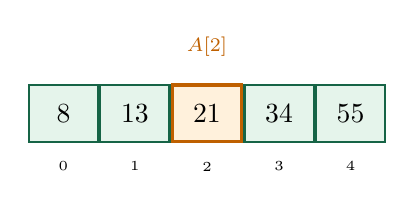
\begin{tikzpicture}[node distance=0pt]
  \node[cell] (c0) {8};
  \node[cell,right=of c0] (c1) {13};
  \node[active,right=of c1] (c2) {21};
  \node[cell,right=of c2] (c3) {34};
  \node[cell,right=of c3] (c4) {55};
  \foreach \x/\lab in {c0/0,c1/1,c2/2,c3/3,c4/4}{
    \node[below=0.12cm of \x,font=\tiny] {\lab};
  }
  \node[above=0.22cm of c2,font=\scriptsize,orange!75!black] {$A[2]$};
\end{tikzpicture}
\end{center}
\begin{alertblock}{Limitation}
Array positions are efficient to access, but inserting into the middle usually
requires shifting following items.
\end{alertblock}
\end{column}
\end{columns}
\end{frame}

\begin{frame}{Dynamic array: grow when capacity is full}
\small
\begin{block}{Why dynamic arrays?}
A fixed-size array cannot grow after its capacity is reached. A dynamic array
allocates a larger block, copies existing references, and continues using the new block.
\end{block}

\begin{center}
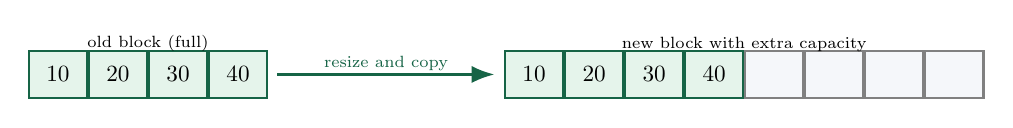
\begin{tikzpicture}[node distance=0pt,scale=0.84,transform shape]
  % old full block on the left
  \node[cell] (a0) at (0,0) {10};
  \node[cell,right=of a0] (a1) {20};
  \node[cell,right=of a1] (a2) {30};
  \node[cell,right=of a2] (a3) {40};
  \node[above=0.22cm of $(a1)!0.5!(a2)$,font=\scriptsize] {old block (full)};

  % new larger block on the right
  \node[cell] (b0) at (7.2,0) {10};
  \node[cell,right=of b0] (b1) {20};
  \node[cell,right=of b1] (b2) {30};
  \node[cell,right=of b2] (b3) {40};
  \node[cell,fill=SoftGray,draw=gray,right=of b3] (b4) {};
  \node[cell,fill=SoftGray,draw=gray,right=of b4] (b5) {};
  \node[cell,fill=SoftGray,draw=gray,right=of b5] (b6) {};
  \node[cell,fill=SoftGray,draw=gray,right=of b6] (b7) {};
  \node[above=0.22cm of $(b3)!0.5!(b4)$,font=\scriptsize] {new block with extra capacity};

  % left-to-right arrow
  \draw[arrow] ([xshift=4pt]a3.east) -- node[above,font=\scriptsize,fill=white,inner sep=1pt]{resize and copy} ([xshift=-4pt]b0.west);
\end{tikzpicture}
\end{center}

\begin{exampleblock}{Python list}
Python's \texttt{list} is implemented as a dynamic array of references. Appending at the end is amortized $O(1)$.
\end{exampleblock}
\end{frame}

\begin{frame}[fragile]{Python list operations: same structure, different costs}
\small
\begin{columns}[T,onlytextwidth]
\begin{column}{0.53\textwidth}
\begin{lstlisting}[language=Python,basicstyle=\ttfamily\scriptsize]
values = [10, 20, 30, 40]

x = values[2]          # index access: O(1)
values.append(50)      # amortized O(1)
last = values.pop()    # O(1)

found = 30 in values   # O(n)
values.insert(0, 5)    # O(n)
values.pop(0)          # O(n)
\end{lstlisting}
\end{column}
\begin{column}{0.43\textwidth}
\begin{block}{Why do front updates cost $O(n)$?}
When an item is inserted or removed near the front, many later references must
shift one position.
\end{block}
\begin{alertblock}{Important distinction}
\texttt{list} is excellent for indexed access and append-at-end, but it is not ideal for frequent front removals.
\end{alertblock}
\end{column}
\end{columns}
\end{frame}

\begin{frame}{Middle insertion in an array requires shifting}
\small
\begin{block}{Task}
Insert $25$ between $20$ and $30$ in an array-based sequence.
\end{block}
\begin{center}
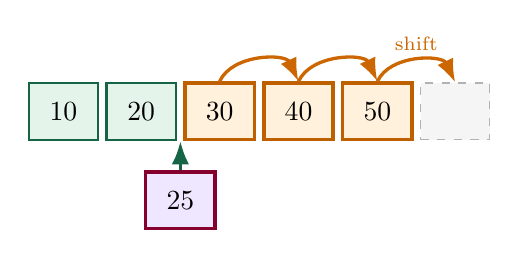
\begin{tikzpicture}[node distance=0.08cm,empty/.style={draw=gray!60,dashed,fill=gray!8,minimum width=0.88cm,minimum height=0.72cm,align=center}]
  \node[cell] (a1) {10};
  \node[cell,right=of a1] (a2) {20};
  \node[active,right=of a2] (a3) {30};
  \node[active,right=of a3] (a4) {40};
  \node[active,right=of a4] (a5) {50};
  \node[empty,right=of a5] (a6) {};
  \draw[orangearrow] (a5.north) to[out=65,in=115] node[midway,above,font=\scriptsize]{shift} (a6.north);
  \draw[orangearrow] (a4.north) to[out=65,in=115] (a5.north);
  \draw[orangearrow] (a3.north) to[out=65,in=115] (a4.north);
  \node[found,below=0.75cm of $(a2)!0.5!(a3)$] (new) {25};
  \draw[arrow] (new.north) -- ($(a2.south)!0.5!(a3.south)$);
\end{tikzpicture}
\end{center}

\begin{alertblock}{Cost}
In the worst case, inserting one item near the front requires moving $\Theta(n)$ existing references.
\end{alertblock}
\end{frame}

% =============================================================
\section{Linked Lists}
% =============================================================

\begin{frame}{Linked-list idea: store nodes and links}
\small
\begin{block}{Core idea}
A linked list stores values in nodes. Each node stores a value and one or more links to neighboring nodes.
The logical order is represented by following links.
\end{block}

\begin{center}
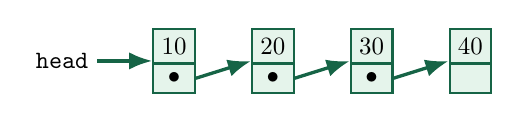
\begin{tikzpicture}[node distance=0.78cm,scale=0.90,transform shape]
  \node (head) {\texttt{head}};
  \node[nodebox,right=of head] (n1) {10\nodepart{second}$\bullet$};
  \node[nodebox,right=of n1] (n2) {20\nodepart{second}$\bullet$};
  \node[nodebox,right=of n2] (n3) {30\nodepart{second}$\bullet$};
  \node[nodebox,right=of n3] (n4) {40\nodepart{second}$\varnothing$};
  \draw[arrow] (head) -- (n1.west);
  \draw[arrow] (n1.second east) -- (n2.west);
  \draw[arrow] (n2.second east) -- (n3.west);
  \draw[arrow] (n3.second east) -- (n4.west);
\end{tikzpicture}
\end{center}

\begin{exampleblock}{Trade-off}
Linked lists avoid shifting values for some updates, but they lose direct indexing.
To reach position $i$, we must follow links from the head.
\end{exampleblock}
\end{frame}

\begin{frame}[fragile]{A node can be represented by a Python class}
\small
\begin{columns}[T,onlytextwidth]
\begin{column}{0.52\textwidth}
\begin{lstlisting}[language=Python,basicstyle=\ttfamily\scriptsize]
class Node:
    def __init__(self, value, next_node=None):
        self.value = value
        self.next = next_node

head = Node(10)
head.next = Node(20)
head.next.next = Node(30)
\end{lstlisting}
\end{column}
\begin{column}{0.44\textwidth}
\begin{center}
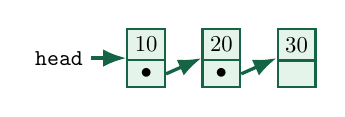
\begin{tikzpicture}[node distance=0.55cm,scale=0.82,transform shape]
  \node (h) {\texttt{head}};
  \node[nodebox,right=of h] (n1) {10\nodepart{second}$\bullet$};
  \node[nodebox,right=of n1] (n2) {20\nodepart{second}$\bullet$};
  \node[nodebox,right=of n2] (n3) {30\nodepart{second}$\varnothing$};
  \draw[arrow] (h) -- (n1.west);
  \draw[arrow] (n1.second east) -- (n2.west);
  \draw[arrow] (n2.second east) -- (n3.west);
\end{tikzpicture}
\end{center}
\begin{alertblock}{Important}
Python does not provide a general-purpose linked-list type as a built-in container. We usually build linked nodes explicitly.
\end{alertblock}
\end{column}
\end{columns}
\end{frame}

\begin{frame}{Types of linked lists}
\scriptsize
\begin{center}
\renewcommand{\arraystretch}{1.16}
\begin{tabular}{L{0.22\textwidth}L{0.29\textwidth}L{0.33\textwidth}}
\toprule
\textbf{Type} & \textbf{Node links} & \textbf{Main idea} \\
\midrule
Singly linked list & \texttt{next} & Traverse from each node to the next node only \\
Doubly linked list & \texttt{prev}, \texttt{next} & Traverse in both directions; deletion can be easier when the node is known \\
Circular linked list & Last node links back to the first node & Useful for cyclic processes such as round-robin scheduling \\
\bottomrule
\end{tabular}
\end{center}

\vspace{0.55em}
\begin{columns}[T,onlytextwidth]
\begin{column}{0.31\textwidth}
\begin{exampleblock}{Singly linked list}
\centering
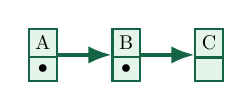
\begin{tikzpicture}[node distance=0.95cm,scale=0.72,transform shape]
  \node[nodebox] (a) {A\nodepart{second}$\bullet$};
  \node[nodebox,right=of a] (b) {B\nodepart{second}$\bullet$};
  \node[nodebox,right=of b] (c) {C\nodepart{second}$\varnothing$};
  \draw[arrow] (a.east) -- (b.west);
  \draw[arrow] (b.east) -- (c.west);
\end{tikzpicture}
\end{exampleblock}
\end{column}\hfill
\begin{column}{0.31\textwidth}
\begin{exampleblock}{Doubly linked list}
\centering
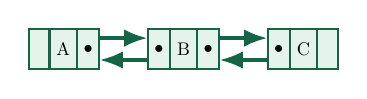
\begin{tikzpicture}[node distance=0.92cm,scale=0.66,transform shape]
  \node[dnode] (a) {$\varnothing$\nodepart{two}A\nodepart{three}$\bullet$};
  \node[dnode,right=of a] (b) {$\bullet$\nodepart{two}B\nodepart{three}$\bullet$};
  \node[dnode,right=of b] (c) {$\bullet$\nodepart{two}C\nodepart{three}$\varnothing$};
  \draw[-Latex,very thick,ForestGreen] ([yshift=6pt]a.east) -- ([yshift=6pt]b.west);
  \draw[-Latex,very thick,ForestGreen] ([yshift=6pt]b.east) -- ([yshift=6pt]c.west);
  \draw[-Latex,very thick,ForestGreen] ([yshift=-6pt]b.west) -- ([yshift=-6pt]a.east);
  \draw[-Latex,very thick,ForestGreen] ([yshift=-6pt]c.west) -- ([yshift=-6pt]b.east);
\end{tikzpicture}
\end{exampleblock}
\end{column}\hfill
\begin{column}{0.31\textwidth}
\begin{exampleblock}{Circular linked list}
\centering
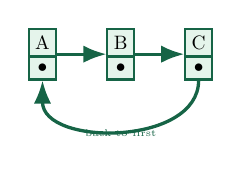
\begin{tikzpicture}[node distance=0.90cm,scale=0.70,transform shape]
  \node[nodebox] (a) {A\nodepart{second}$\bullet$};
  \node[nodebox,right=of a] (b) {B\nodepart{second}$\bullet$};
  \node[nodebox,right=of b] (c) {C\nodepart{second}$\bullet$};
  \draw[arrow] (a.east) -- (b.west);
  \draw[arrow] (b.east) -- (c.west);
  \draw[arrow] (c.south) .. controls +(0,-1.2) and +(0,-1.2) .. (a.south);
  \node[below=0.78cm of b,font=\tiny,ForestGreen] {back to first};
\end{tikzpicture}
\end{exampleblock}
\end{column}
\end{columns}
\end{frame}

\begin{frame}{Singly linked list: operation overview}
\scriptsize
\begin{center}
\renewcommand{\arraystretch}{1.05}
\begin{tabular}{L{0.30\textwidth}L{0.42\textwidth}c}
\toprule
\textbf{Operation} & \textbf{Idea} & \textbf{Cost} \\
\midrule
Traverse / search & Follow \texttt{next} links from \texttt{head} & $O(n)$ \\
Prepend & \texttt{new.next = head}; update \texttt{head} & $O(1)$ \\
Insert after known node & Save old successor; redirect two links & $O(1)$ \\
Delete after known predecessor & Predecessor skips the removed node & $O(1)$ \\
Append with only \texttt{head} & Traverse to the last node, then attach new node & $O(n)$ \\
Append with \texttt{head} and \texttt{tail} & Attach after old tail; update \texttt{tail} & $O(1)$ \\
\bottomrule
\end{tabular}
\end{center}

\vspace{0.4em}
\begin{block}{Important qualification}
$O(1)$ linked-list update means the correct node or predecessor is already known. Locating it may still cost $O(n)$.
\end{block}
\end{frame}

% =============================================================
\section{Traversing and Updating a Singly Linked List}
% =============================================================

\begin{frame}[fragile]{Traversal follows links until the target or \texttt{NONE}}
\begin{columns}[T]
\begin{column}{0.58\textwidth}
\begin{lstlisting}[style=pseudonumbered]
FUNCTION LINKED_SEARCH(head, target)
INPUT: first node and target value
OUTPUT: first matching node, or NONE
    current = head
    WHILE current != NONE DO
        IF current.value == target THEN
            RETURN current
        current = current.next
    RETURN NONE
\end{lstlisting}
\end{column}
\begin{column}{0.38\textwidth}
\begin{block}{Invariant}
Before each iteration, every node before \texttt{current} has already been examined and does not contain the target.
\end{block}
\begin{exampleblock}{Complexity}
Best case $\Theta(1)$; worst case $\Theta(n)$. Only one traversal reference is required, so auxiliary space is $\Theta(1)$.
\end{exampleblock}
\end{column}
\end{columns}
\end{frame}

\begin{frame}{Prepending changes only two references}
\small
\begin{columns}[T,onlytextwidth]
\begin{column}{0.56\textwidth}
\begin{center}
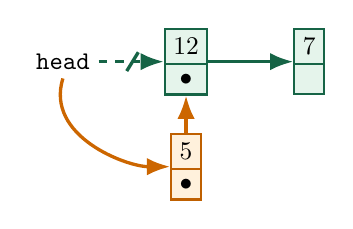
\begin{tikzpicture}[scale=0.92,transform shape]
  \node (head) at (-0.7,1.0) {\texttt{head}};
  \node[nodebox] (n1) at (1.0,1.0) {12\nodepart{second}$\bullet$};
  \node[nodebox] (n2) at (2.7,1.0) {7\nodepart{second}$\varnothing$};
  \node[nodebox,fill=SoftOrange,draw=orange!75!black] (new) at (1.0,-0.45) {5\nodepart{second}$\bullet$};
  % unchanged link
  \draw[arrow] (n1.east) -- (n2.west);
  % replaced old head link: dashed with a slash mark
  \draw[dashed,very thick,ForestGreen,-Latex] (head.east) -- (n1.west);
  \draw[ForestGreen,very thick] ($(head.east)!0.52!(n1.west)+(0.08,0.13)$) -- ($(head.east)!0.52!(n1.west)+(-0.08,-0.13)$);
  % new links being created
  \draw[orangearrow] (new.north) -- (n1.south);
  \draw[orangearrow] (head.south) .. controls +(-0.25,-0.80) and +(-0.60,0.00) .. (new.west);
\end{tikzpicture}
\end{center}
\end{column}
\begin{column}{0.40\textwidth}
\begin{exampleblock}{Correct update order}
\begin{enumerate}
  \item \texttt{new.next = head}
  \item \texttt{head = new}
\end{enumerate}
\end{exampleblock}
\begin{block}{Cost}
Prepending takes $\Theta(1)$ time because it does not shift or traverse existing nodes.
\end{block}
\end{column}
\end{columns}
\begin{alertblock}{Lost-list error}
Replacing \texttt{head} before saving the old head as \texttt{new.next} disconnects the old list.
\end{alertblock}
\end{frame}

\begin{frame}{Insert after a known node without shifting values}
\small
\begin{columns}[T,onlytextwidth]
\begin{column}{0.59\textwidth}
\begin{center}
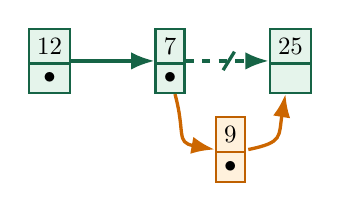
\begin{tikzpicture}[scale=0.90,transform shape]
  \node[nodebox] (a) at (0.0,0.9) {12\nodepart{second}$\bullet$};
  \node[nodebox] (b) at (1.7,0.9) {7\nodepart{second}$\bullet$};
  \node[nodebox] (c) at (3.4,0.9) {25\nodepart{second}$\varnothing$};
  \node[nodebox,fill=SoftOrange,draw=orange!75!black] (new) at (2.55,-0.35) {9\nodepart{second}$\bullet$};
  % unchanged link
  \draw[arrow] (a.east) -- (b.west);
  % replaced old successor link: dashed with a slash mark
  \draw[dashed,very thick,ForestGreen,-Latex] (b.east) -- (c.west);
  \draw[ForestGreen,very thick] ($(b.east)!0.52!(c.west)+(0.08,0.13)$) -- ($(b.east)!0.52!(c.west)+(-0.08,-0.13)$);
  % new links being created (routed to avoid overlapping nodes)
  \draw[orangearrow] ([xshift=2pt]b.south) .. controls +(0.15,-0.55) and +(-0.55,0.10) .. (new.west);
  \draw[orangearrow] ([xshift=1pt]new.east) .. controls +(0.50,0.10) and +(-0.10,-0.60) .. ([xshift=-2pt]c.south);
\end{tikzpicture}
\end{center}
\end{column}
\begin{column}{0.37\textwidth}
\begin{exampleblock}{Correct update order}
For known node \texttt{current}:
\begin{enumerate}
  \item \texttt{new.next = current.next}
  \item \texttt{current.next = new}
\end{enumerate}
\end{exampleblock}
\begin{block}{Cost}
The link update takes $\Theta(1)$ once \texttt{current} is known.
\end{block}
\end{column}
\end{columns}
\begin{alertblock}{Why the order matters}
Save the old successor before replacing \texttt{current.next}; otherwise the remaining suffix may become unreachable.
\end{alertblock}
\end{frame}


\begin{frame}{Delete a node by bypassing it}
\small
\begin{columns}[T,onlytextwidth]
\begin{column}{0.59\textwidth}
\begin{center}
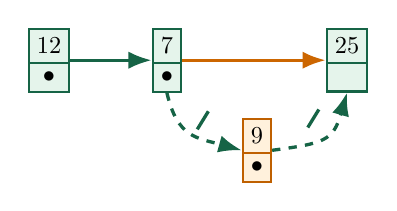
\begin{tikzpicture}[scale=0.88,transform shape]
  \node[nodebox] (a) at (0.0,1.05) {12\nodepart{second}$\bullet$};
  \node[nodebox] (prev) at (1.7,1.05) {7\nodepart{second}$\bullet$};
  \node[nodebox] (next) at (4.3,1.05) {25\nodepart{second}$\varnothing$};
  \node[nodebox,fill=SoftOrange,draw=orange!75!black] (del) at (3.0,-0.25) {9\nodepart{second}$\bullet$};

  % unchanged link
  \draw[arrow] (a.east) -- (prev.west);

  % old links through the deleted node: dashed with slash marks
  \draw[dashed,very thick,ForestGreen,-Latex] (prev.south) .. controls +(0.15,-0.65) and +(-0.65,0.18) .. (del.west);
  \draw[ForestGreen,very thick] ($(prev.south)!0.48!(del.west)+(0.08,0.13)$) -- ($(prev.south)!0.48!(del.west)+(-0.08,-0.13)$);
  \draw[dashed,very thick,ForestGreen,-Latex] (del.east) .. controls +(0.75,0.10) and +(-0.20,-0.70) .. (next.south);
  \draw[ForestGreen,very thick] ($(del.east)!0.55!(next.south)+(0.08,0.13)$) -- ($(del.east)!0.55!(next.south)+(-0.08,-0.13)$);

  % new bypass link
  \draw[orangearrow] (prev.east) -- (next.west);
\end{tikzpicture}
\end{center}
\end{column}
\begin{column}{0.37\textwidth}
\begin{exampleblock}{Known references}
\texttt{previous} points to node 7.\\
\texttt{current} points to node 9.
\end{exampleblock}
\begin{block}{Link update}
\[
\texttt{previous.next = current.next}
\]
Node 9 is bypassed and becomes unreachable from \texttt{head}.
\end{block}
\end{column}
\end{columns}
\begin{alertblock}{Important distinction}
Finding the node may take $O(n)$ time, but the bypass link update itself is $O(1)$.
\end{alertblock}
\end{frame}

\begin{frame}[fragile]{Delete the first occurrence by tracking its predecessor}
\begin{columns}[T]
\begin{column}{0.62\textwidth}
\begin{lstlisting}[style=pseudonumbered]
FUNCTION DELETE_FIRST(head, target)
INPUT: head and target value
OUTPUT: possibly updated head
    IF head == NONE THEN RETURN NONE
    IF head.value == target THEN
        RETURN head.next
    previous = head
    current = head.next
    WHILE current != NONE DO
        IF current.value == target THEN
            previous.next = current.next
            RETURN head
        previous = current
        current = current.next
    RETURN head
\end{lstlisting}
\end{column}
\begin{column}{0.34\textwidth}
\begin{block}{Special case}
Deleting the first node changes \texttt{head}; deleting a later node changes its predecessor's \texttt{next} link.
\end{block}
\begin{exampleblock}{Complexity}
Finding the value is worst-case $\Theta(n)$. Once the node and predecessor are known, unlinking takes $\Theta(1)$.
\end{exampleblock}
\end{column}
\end{columns}
\end{frame}

\begin{frame}{Head and tail references}
\small
\begin{block}{Why keep a tail reference?}
A singly linked list with only a head reference must traverse to find the last node before appending. A list with both head and tail can append in constant time.
\end{block}

\begin{center}
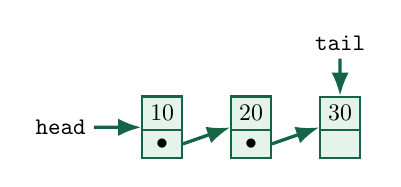
\begin{tikzpicture}[node distance=0.70cm,scale=0.86,transform shape]
  \node (head) at (0,0.75) {\texttt{head}};
  \node[nodebox,right=of head] (n1) {10\nodepart{second}$\bullet$};
  \node[nodebox,right=of n1] (n2) {20\nodepart{second}$\bullet$};
  \node[nodebox,right=of n2] (n3) {30\nodepart{second}$\varnothing$};
  \node[above=0.55cm of n3] (tail) {\texttt{tail}};
  \draw[arrow] (head) -- (n1.west);
  \draw[arrow] (n1.second east) -- (n2.west);
  \draw[arrow] (n2.second east) -- (n3.west);
  \draw[arrow] (tail) -- (n3.north);
\end{tikzpicture}
\end{center}

\begin{exampleblock}{Append with a tail}
Create a new node, set \texttt{tail.next} to it, then update \texttt{tail}. If the list was empty, update both \texttt{head} and \texttt{tail}.
\end{exampleblock}
\end{frame}

% =============================================================
\section{Comparing Array-Based and Linked Structures}
% =============================================================

\begin{frame}{Array-based lists and linked lists make different trade-offs}
\scriptsize
\begin{center}
\renewcommand{\arraystretch}{1.20}
\begin{tabular}{L{0.28\textwidth}cc}
\toprule
\textbf{Operation / property} & \textbf{Python list / dynamic array} & \textbf{Singly linked list} \\
\midrule
Access position $i$ & $O(1)$ & $O(i)$, worst-case $O(n)$ \\
Search by value & $O(n)$ & $O(n)$ \\
Add at end & Amortized $O(1)$ & $O(1)$ with tail; otherwise $O(n)$ \\
Add at front & $O(n)$ & $O(1)$ \\
Delete front & $O(n)$ & $O(1)$ \\
Insert after a known node & $O(n)$ shifting & $O(1)$ link update \\
Extra storage per value & Low & One or more links \\
Memory locality & Good, contiguous references & Usually weaker, nodes may be scattered \\
\bottomrule
\end{tabular}
\end{center}
\begin{alertblock}{No structure wins every workload}
Choose the representation from the operations that dominate the application.
\end{alertblock}
\end{frame}

\begin{frame}{Decision guide: array or linked list?}
\small
\begin{columns}[T,onlytextwidth]
\begin{column}{0.48\textwidth}
\begin{exampleblock}{Prefer array-based lists when}
\begin{itemize}
  \item indexed access is frequent;
  \item append-at-end is common;
  \item memory overhead should be small;
  \item cache-friendly traversal matters.
\end{itemize}
\end{exampleblock}
\end{column}
\begin{column}{0.48\textwidth}
\begin{alertblock}{Prefer linked structures when}
\begin{itemize}
  \item insert/delete after known nodes is frequent;
  \item front updates are frequent;
  \item the structure is used to implement another ADT;
  \item direct indexing is not important.
\end{itemize}
\end{alertblock}
\end{column}
\end{columns}

\begin{block}{Practical note}
In Python application code, built-in containers are usually preferred. Linked lists are still important for understanding pointers/references, representation trade-offs, and many data-structure implementations.
\end{block}
\end{frame}

\begin{frame}{Self-check: arrays and linked lists}
\small
\begin{enumerate}
  \item Why is $A[i]$ constant time in an array-based representation?
  \item Why can inserting at index $0$ in a Python list cost $O(n)$?
  \item In a singly linked list, why does accessing position $i$ cost $O(i)$?
  \item What does ``insert after a known node is $O(1)$'' really assume?
  \item Which references change when prepending a node to a non-empty linked list?
  \item Why can a tail reference make append $O(1)$?
\end{enumerate}
\begin{block}{Discussion rule}
For each answer, name the representation first, then state the operation cost.
\end{block}
\end{frame}

\begin{frame}{Integrated activity: choose the representation}
\small
\begin{block}{Scenarios}
Choose between an array-based list and a linked representation. Justify your choice by naming the dominant operation.
\end{block}
\begin{columns}[T,onlytextwidth]
\begin{column}{0.55\textwidth}
\begin{enumerate}
  \item Store daily sales values and frequently access day $i$.
  \item Maintain a waiting list where people are often removed from the front.
  \item Build a sequence by repeatedly appending new observations.
  \item Insert many items after a known cursor position.
  \item Search for a value without knowing its position.
\end{enumerate}
\end{column}
\begin{column}{0.41\textwidth}
\begin{alertblock}{Answer format}
For each case, state:
\begin{enumerate}
  \item the representation;
  \item the important operation;
  \item the expected or worst-case cost.
\end{enumerate}
\end{alertblock}
\end{column}
\end{columns}
\end{frame}

\begin{frame}{Key takeaways}
\small
\begin{itemize}
  \item A sequence is a logical order; arrays and linked lists are different ways to represent it.
  \item Arrays support direct indexing because positions are computed from a base address.
  \item Python lists are dynamic arrays of references; append is amortized $O(1)$, while front insert/delete is $O(n)$.
  \item Linked lists connect nodes with links; traversal is sequential rather than direct.
  \item Linked updates can be $O(1)$ only after the correct node or predecessor is known.
  \item Singly, doubly, and circular linked lists differ by the links each node stores and the traversal patterns they support.
\end{itemize}
\end{frame}

\begin{frame}{After-class practice}
\small
\begin{enumerate}
  \item Draw the memory diagram for a Python list storing five integers.
  \item Trace insertion at index $0$ in an array-based list of length $6$.
  \item Define a Python \texttt{Node} class and manually create a three-node linked list.
  \item Write pseudocode to count nodes in a singly linked list.
  \item Write pseudocode to append using both \texttt{head} and \texttt{tail} references.
  \item Compare array-based and linked representations for a playlist editor.
\end{enumerate}
\end{frame}

\end{document}
